\documentclass[epsfig,10pt,fullpage]{article}

\newcommand{\LabNum}{1}
\newcommand{\CommonDocsPath}{../../../common/docs}
\addtolength{\textwidth}{1.5in}
\addtolength{\oddsidemargin}{-0.75in}
\addtolength{\topmargin}{-0.75in}
\addtolength{\textheight}{1.5in}
\addtolength{\evensidemargin}{0.75in}
\setlength\parindent{0pt}
\raggedbottom

\usepackage{ae,aecompl}
\usepackage{epsfig,float,times}
\usepackage[hypcap]{caption}
\usepackage[pdftex, colorlinks]{hyperref}
\usepackage{graphicx}
\usepackage[usenames, dvipsnames]{color}
\usepackage{rotating}
\usepackage{tikz}
\usetikzlibrary{automata,positioning}
\usepackage{placeins}

\widowpenalty 10000
\clubpenalty 10000

\newcommand{\red}[1]{{\color{red}\sf{#1}}}
\newcommand{\green}[1]{{\color{green}\sf{#1}}}
\newcommand{\blue}[1]{{\color{blue}\sf{#1}}}
\definecolor{PineGreen}{rgb}{0.0, 0.47, 0.44}
\definecolor{ForestGreen}{rgb}{0.13, 0.55, 0.13}
\definecolor{Brown}{rgb}{0.59, 0.29, 0.0}

\newcommand{\UPDatePublished}{Oct 2021}
\newcommand{\versnum}{21.1} %version number quartus/AMP
\newcommand{\quartusname}{Quartus\textsuperscript{\textregistered} Prime}	
\newcommand{\UPTextBar}{For \quartusname{} \versnum{}}
\newcommand{\thisyear}{2021 } %for copyright
\newcommand{\company}{FPGAcademy.org}
\newcommand{\longteamname}{FPGAcademy.org}
\newcommand{\teamname}{FPGAcademy}
\newcommand{\website}{FPGAcademy.org}

\newcommand{\productAcronym}{AMP}
\newcommand{\productNameShort}{Monitor Program}

\newcommand{\productNameMedTM}{A Monitor Program}
\newcommand{\productNameMed}{A Monitor Program}

%\newcommand{\headerLogoFilePath}[1]{#1/FPGAcademy.png}

% listings is a package that supports encapsulating source code in LaTeX conveniently
\usepackage{listings}

\def\expandparam\lstinputlisting[#1]#2{\edef\tmp{\noexpand\lstinputlisting[#1]{#2}}\tmp}

%%%%%%%%%%%%%%%%%%%% Source Code Formatting %%%%%%%%%%%%%%%%%%%%
\definecolor{globalCommentColour}{rgb}{0.588,0.588,0.588}

%%%%%%%%%%%%%%%%%%%%%%%%%%%%%%%%%%%%%%%%%%%%%%%%%%%%
% Defining language style
% NiosII ASM
\lstdefinelanguage[NiosII]{Assembler} {
  morekeywords={add, addi, and, andhi, andi, beq, bge, bgeu, bgt, bgtu, ble,  bleu, blt, bltu, bne, br, break,
  bret, call, callr, cmpeq, cmpeqi, cmpge, cmpgei, cmpgeu, cmpgeui, cmpgt, cmpgti, cmpgtu, cmpgtui, cmple,
  cmplei, cmpleu, cmpleui, cmplt, cmplti, cmpltu, cmpltui, cmpne, cmpnei, custom, div, divu, eret, flushd,
  flushda, flushi, flushp, initd, initda, initi, jmp, jmpi, ldb, ldbio, ldbu, ldbuio, ldh, ldhio, ldhu, ldhuio,
  ldw, ldwio, mov, movhi, movi, movia, movui, mul, muli, mulxss, mulxsu, mulxuu, nextpc, nop, nor, or, orhi, ori,
  rdctl, rdprs, ret, rol, roli, ror, sll, slli, sra, srai, srl, srli, stb, stbio, sth, sthio, stw, stwio,
  sub, subi, sync, trap, wrctl, wrtcl, wrprs, xor, xori, xorhi, xori},
  morekeywords=[2]{.abort, .ABORT, .align, .app-file, .ascii, .asciz, .balign, .byte, .comm, .data, .def,
  .desc, .dim, .double, .eject, .else, .end, .endef, .endif, .equ, .equiv, .err, .extern, .file, .fill, .float,
  .global, .globl, .hword, .ident, .if, .include, .int, .irp, .irpc, .lcomm, .lflags, .line, .linkonce, .ln,
  .list, .long, .macro, .mri, .nolist, .octa, .org, .p2align, .psize, .quad, .rept, .sbttl, .scl, .section,
  .set, .short, .single, .size, .sleb128, .skip, .space, .stadb, .stabn, .stabs, .string, .symver, .tag,
  .text, .title, .type, .val, .uleb128, .word},
  morekeywords=[3]{et, bt, gp, sp, fp, ea, sstatus, ra, pc, status, estatus, bstatus, ienable, ipending, cpuid,
  exception, pteaddr, tlbacc, tlbmisc, eccinj, badaddr, config, mpubase, mpuacc},
  sensitive=t,
  alsoletter=.,
  morestring=[b]",
  morecomment=[s]{/*}{*/},
  morecomment=[l]\#,
}[keywords,comments,strings]
   
%% NOTE: morekeywords=[2] are GNU directives.
   
\definecolor{niosInstructionColour}{rgb}{0.000,0.608,0.000}
\definecolor{niosDirectiveColour}{rgb}{0.000,0.000,0.902}
\definecolor{niosSpecialRegColour}{rgb}{0.000,0.000,0.000}
\definecolor{niosStringColour}{rgb}{0.808,0.482,0.000}
   
%% NOTE: To make bold use: =\bfseries\color{<colour>}
\lstdefinestyle{defaultNiosStyle} {
  language=[NiosII]{Assembler},
  stringstyle=\color{niosStringColour},
  keywordstyle=\color{niosInstructionColour},
  keywordstyle=[2]\color{niosDirectiveColour},
  keywordstyle=[3]\itshape\color{niosSpecialRegColour}
}
%%%%%%%%%%%%%%%%%%%%%%%%%%%%%%%%%%%%%%%%%%%%%%%%%%%%

%%%%%%%%%%%%%%%%%%%%%%%%%%%%%%%%%%%%%%%%%%%%%%%%%%%%
% Defining language style
% ArmA9 ASM
\lstdefinelanguage[ArmA9]{Assembler} {
  morekeywords={ADC, ADD, ADDS, AND, ANDS, B, BAL, BEQ, BGE, BGT, BL, BLT, BIC, BKPT, BLX, BNE, BX, CDP, CLZ, CMN, CMP, EOR,
  EORS, LDC, LDM, LDR, LDRB, LDRBT, LDRH, LDRSB, LDRSH, LDRT, LSL, MCR, MLA, MOV, MOVW, MOVT, MRC, MRS, MSR, MUL, MVN, ORR, PLD,
  ROR, RSB, RSC, SBC, SMLAL, SMULL, STC, STM, STR, STRB, STRBT, STRH, STRT, SUB, SUBS, SWI, SWP, SWPB, TEQ, UMLAL,
  PUSH, POP, MOVS, RORS, LSR},
  morekeywords=[2]{.abort, .ABORT, .align, .app-file, .ascii, .asciz, .balign, .byte, .comm, .data, .def,
  .desc, .dim, .double, .eject, .else, .end, .endef, .endif, .equ, .equiv, .err, .extern, .file, .fill, .float,
  .global, .globl, .hword, .ident, .if, .include, .int, .irp, .irpc, .lcomm, .lflags, .line, .linkonce, .ln,
  .list, .long, .macro, .mri, .nolist, .octa, .org, .p2align, .psize, .quad, .rept, .sbttl, .scl, .section,
  .set, .short, .single, .size, .sleb128, .skip, .space, .stadb, .stabn, .stabs, .string, .symver, .tag,
  .text, .title, .type, .val, .vectors, .uleb128, .word},
  morekeywords=[3]{SP, PC, MIDR, CTR, TCMTR, TLBTR, MPIDR, ID_PFR0, ID_PFR1, ID_DFR0, ID_MMFR0, ID_MMFR1, ID_MMFR2,
  ID_MMFR3, ID_ISAR0, ID_ISAR1, ID_ISAR2, ID_ISAR3, ID_ISAR4, CCSIDR, CLIDR, AIDR, CSSELR, TTBR0, TTRB1, TTBR2, DACR,
  DFSR, IFSR, ADFSR, AIFSR, DFAAR, IFAR, ICIALLUIS, BPIALLIS, PAR, ICIALLU, ICIMVAU, BPIALL, DCIMVAC, DCISW, V2PCWPR,
  DCCVAC, DCCSW, DDIMVAC, DCISW, TLBALLIS, TLBIMVAIS, TLBIASIDIS, TLBIMVAAIS, TLBIALL, TLBIMVA, TLBIASID, TLBIMVAA,
  PMCR, PMCNTENSET, PMCNTENCLR, PMOVSR, PMSWINC, PMSELR, PMXEVTYPER, PMXEVCNTR, PMUSERENR, PMINTENSET, PMINTENCLR,
  PRRR, NRRR, PLEIDR, PLEASR, PLEFSR, PLEUAR, PLEPCR, VBAR, MVBAR, ISR, FCSEIDR, CONTEXTIDR, TPIDRURW, TPIDRURO, TPIDRPRW},
  sensitive=f,
  alsoletter=.,
  morestring=[b]",
  morecomment=[s]{/*}{*/},
  morecomment=[l]{//},
}[keywords,comments,strings]
   
%% NOTE: morekeywords=[2] are GNU directives.
   
\definecolor{armInstructionColour}{rgb}{0.000,0.608,0.000}
\definecolor{armDirectiveColour}{rgb}{0.000,0.000,0.902}
\definecolor{armSpecialRegColour}{rgb}{0.000,0.000,0.000}
\definecolor{armStringColour}{rgb}{0.808,0.482,0.000}
   
\lstdefinestyle{defaultArmStyle} {
  language=[ArmA9]{Assembler},
  stringstyle=\color{armStringColour},
  keywordstyle=\color{armInstructionColour},
  keywordstyle=[2]\color{armDirectiveColour},
  keywordstyle=[3]\itshape\color{armSpecialRegColour}
}
%%%%%%%%%%%%%%%%%%%%%%%%%%%%%%%%%%%%%%%%%%%%%%%%%%%%

%%%%%%%%%%%%%%%%%%%%%%%%%%%%%%%%%%%%%%%%%%%%%%%%%%%%
% Defining language style
% FPGAcademy ASM
\lstdefinelanguage{ASM}{
  morekeywords = [1]{mv, mvt, mvne, mvcc, add, sub, st, ld, and, b, bne, beq, bcc, bcs},
  morekeywords = [2]{word, define},
  keywordstyle = [1]\color{ForestGreen},
  keywordstyle = [2]\color{blue},
  sensitive = true,
  morecomment = [l]{//},
}

\lstset{
  language = ASM,
  basicstyle=\small\color{black}\ttfamily,
  commentstyle=\small\color{Brown}\itshape\ttfamily,
  showstringspaces=false,
  frame=none, %lines % boxed listings
  breaklines=true,
  breakatwhitespace=true,
  tabsize=3
}
%%%%%%%%%%%%%%%%%%%%%%%%%%%%%%%%%%%%%%%%%%%%%%%%%%%%

%%%%%%%%%%%%%%%%%%%%%%%%%%%%%%%%%%%%%%%%%%%%%%%%%%%%
% Defining language style
% Java
\definecolor{javaStringColour}{rgb}{0.808,0.482,0}
%%%%%%%%%%%%%%%%%%%%%%%%%%%%%%%%%%%%%%%%%%%%%%%%%%%%

%%%%%%%%%%%%%%%%%%%%%%%%%%%%%%%%%%%%%%%%%%%%%%%%%%%%
% Defining language style
% C
\definecolor{CStringColour}{rgb}{0.808,0.482,0}

\lstset{
  language = C,
  basicstyle=\small\color{black}\ttfamily, 
  commentstyle=\small\color{PineGreen}\itshape\ttfamily,
  keywordstyle=\small\color{blue}\bfseries\ttfamily,
  showstringspaces=false,
  frame=none, %lines % boxed listings
  breaklines=true,
  breakatwhitespace=true,
  tabsize=3
}
%%%%%%%%%%%%%%%%%%%%%%%%%%%%%%%%%%%%%%%%%%%%%%%%%%%%

%%%%%%%%%%%%%%%%%%%%%%%%%%%%%%%%%%%%%%%%%%%%%%%%%%%%
% Defining language style
% Verilog
\definecolor{verilogCommentColour}{rgb}{0.000,0.502,0.000}

\lstdefinestyle{defaultVerilogStyle} {
  language={Verilog},
  keywordstyle=\color{blue},
  commentstyle=\color{verilogCommentColour}
}
%%%%%%%%%%%%%%%%%%%%%%%%%%%%%%%%%%%%%%%%%%%%%%%%%%%%

%%%%%%%%%%%%%%%%%%%%%%%%%%%%%%%%%%%%%%%%%%%%%%%%%%%%
% Defining language style
% VHDL
\lstdefinestyle{defaultVHDLStyle} {
  language={VHDL},
  keywordstyle=\color{blue},
  commentstyle=\color{verilogCommentColour}
}
%%%%%%%%%%%%%%%%%%%%%%%%%%%%%%%%%%%%%%%%%%%%%%%%%%%%

%%%%%%%%%%%%%%%%%%%%%%%%%%%%%%%%%%%%%%%%%%%%%%%%%%%%
% Defining language style
% LaTeX
\lstdefinelanguage[LocalLaTeX]{TeX}[LaTeX]{TeX}{moretexcs={bf, it, sf, lstset},}

\lstdefinestyle{defaultLocalLatexStyle} {
  language=[LocalLatex]{TeX},
  keywordstyle=\color{blue}\bfseries,
  keywordstyle=[2]\color{blue},
  keywordstyle=[3]\color{blue}\bfseries
}
%%%%%%%%%%%%%%%%%%%%%%%%%%%%%%%%%%%%%%%%%%%%%%%%%%%%

%%%%%%%%%%%%%%%%%%%%%%%%%%%%%%%%%%%%%%%%%%%%%%%%%%%%
% Defining language style
% Default
\lstset{
  basicstyle=\small\color{black}\ttfamily,
  commentstyle=\small\color{globalCommentColour}\itshape\ttfamily,
  keywordstyle=\small\color{blue}\bfseries\ttfamily,
  showstringspaces=false,
  frame=none, %lines % boxed listings
  breaklines=true,
  breakatwhitespace=true,
  tabsize=3
}
%%%%%%%%%%%%%%%%%%%%%%%%%%%%%%%%%%%%%%%%%%%%%%%%%%%%


\hypersetup{
  pdftitle={Digital Logic Lab Exercise \LabNum},
  linkcolor=blue,
  hyperindex=true,
  pdfauthor={FPGAcademy.org},
  pdfkeywords={FPGAcademy.org, FPGAcademy, Lab, Exercise, Digital Logic},
  bookmarks,
  bookmarksopen=false,
  filecolor=blue,
  pdfstartview={FitH},
  urlcolor=blue,
  plainpages=false,
  pdfpagelabels=true,
  linkbordercolor={1 1 1} %no color for link border
}



\begin{document}

\centerline{\huge Digital Logic}
~\\
\centerline{\huge Laboratory Exercise \LabNum}
~\\
\centerline{\large Switches, Lights, and Multiplexers}
~\\

The purpose of this exercise is to learn how to connect simple input and
output devices to an FPGA chip and implement a circuit that uses these devices.
We will use the switches on the DE-series boards as inputs to the circuit.
We will use light emitting diodes (LEDs) and 7-segment displays as output
devices.

\section*{Part I}
\addcontentsline{toc}{1}{Part I}
The DE10-Lite, DE0-CV, and DE1-SoC boards provide ten switches and lights, called 
{\it SW}$_{9-0}$ and {\it LEDR}$_{9-0}$. Similarly, the DE2-115 provides eighteen switches 
and lights. The switches can be used to provide inputs, and the lights can be used as 
output devices. Figure~\ref{fig:1} shows a simple Verilog module that uses ten switches 
and shows their states on the LEDs. Since there are multiple switches and lights
it is convenient to represent them as vectors in the Verilog code, as shown. We have used a
single assignment statement for all {\it LEDR} outputs, which is equivalent to the 
individual assignments:

\begin{center}
\begin{minipage}[t]{12.5 cm}
\begin{tabbing}
$\ldots$\\
{\bf assign} LEDR[2] = SW[2];\\
{\bf assign} LEDR[1] = SW[1];\\
{\bf assign} LEDR[0] = SW[0];
\end{tabbing}
\end{minipage}
\end{center}

The DE-series boards have hardwired connections between its FPGA chip and the switches and
lights. To use the switches and lights it is necessary to include in
your Quartus\textsuperscript{\textregistered} project the correct pin assignments, which are 
given in your board's user manual. For example, the DE1-SoC manual specifies that 
{\it SW}$_0$ is connected to the FPGA pin {\it AB12} and {\it LEDR}$_0$ is connected to 
pin {\it V16}. A good way to make the required pin assignments is to import into the 
Quartus software the pin assignment file for your board, which is provided on the 
Boards section of FPGAcademic.org web site. The procedure for making pin assignments is 
described in the tutorial {\it Quartus Introduction using Verilog Design}, which is 
also available from FPGAcademic.org.
~\\

It is important to realize that the pin assignments in the
file are useful only if the pin names that appear in this file
are exactly the same as the port names used in your Verilog module.
For example, if the pin assignment file uses the names {\it SW}[0], $\ldots$, {\it SW}[9] 
and {\it LEDR}[0], $\ldots$, {\it LEDR}[9], then these are the names that must be used
for input and output ports in the Verilog code, as we have done in Figure~\ref{fig:1}.

~\\
~\\
\begin{figure}[H]
\begin{center}
\begin{minipage}[t]{12.5 cm}
\begin{tabbing}
ZZ\=ZZ\=ZZ\=ZZ\=ZZ\=ZZ\=ZZ\=ZZ\=ZZ\=ZZ\=ZZ\kill
// Module that connects ten switches and lights\\
{\bf module} ~part1 (SW, LEDR);\\
\>{\bf input} [9:0] SW;\>\>\>\>\>\>\>\>// slide switches\\
\>{\bf output} [9:0] LEDR;\>\>\>\>\>\>\>\>// red LEDs\\
~\\
\>{\bf assign} LEDR = SW;\\
{\bf endmodule}
\end{tabbing}
\end{minipage}
	\caption{Verilog code that uses ten switches and lights.}
	\label {fig:1}
\end{center}
\end{figure}

\newpage
Perform the following steps to implement a circuit corresponding to the code
in  Figure~\ref{fig:1} on the DE-series boards.
\begin{enumerate}
\item Create a new Quartus project for your circuit. Select the target chip that corresponds to your DE-series board.
Refer to Table \ref{tab:device} for a list of devices.
\item Create a Verilog module for the code in  Figure~\ref{fig:1} and include it in your project.
\item Include in your project the required pin assignments for your DE-series board, as discussed
above. Compile the project.
\item Generate a .qsf file in Quartus and upload it to the NO-IDE lab of LabsLand. Test the functionality of the 
circuit by toggling the switches and observing the LEDs.
\item For more info, if you have a FPGA chip, you can download the compiled circuit into the FPGA chip by using the Quartus Programmer tool (the procedure
	for using the Programmer tool is described in the tutorial Quartus Introduction). 
\end{enumerate}

\begin{table}[H]
	\begin{center}
	\begin{tabular}{l | l}
   \bf{Board} & \bf{Device Name} \\
	\hline
	\rule{0pt}{3ex}DE10-Lite & MAX\textsuperscript{\textregistered} 10 10M50DAF484C6GES \\
	DE0-CV & Cyclone\textsuperscript{\textregistered} V 5CEBA4F23C7 \\
	DE1-SoC & Cyclone\textsuperscript{\textregistered} V SoC 5CSEMA5F31C6 \\
	DE2-115 & Cyclone\textsuperscript{\textregistered} IVE EP4CE115F29C7 \\
	\end{tabular}
	\end{center}
	\caption{DE-series FPGA device names}
	\label{tab:device}
\end{table}

\section*{Part II}
\addcontentsline{toc}{2}{Part II}
Figure~\ref{fig:2}$a$ shows a sum-of-products circuit that implements
a 2-to-1 {\it multiplexer} with a select input $s$.
If $s = 0$ the multiplexer's output $m$ is equal to the input $x$, and if $s=1$ the
output is equal to $y$. Part $b$ of the figure gives a truth table for this
multiplexer, and part $c$ shows its circuit symbol. 

\begin{figure}[H]
	\begin{center}
		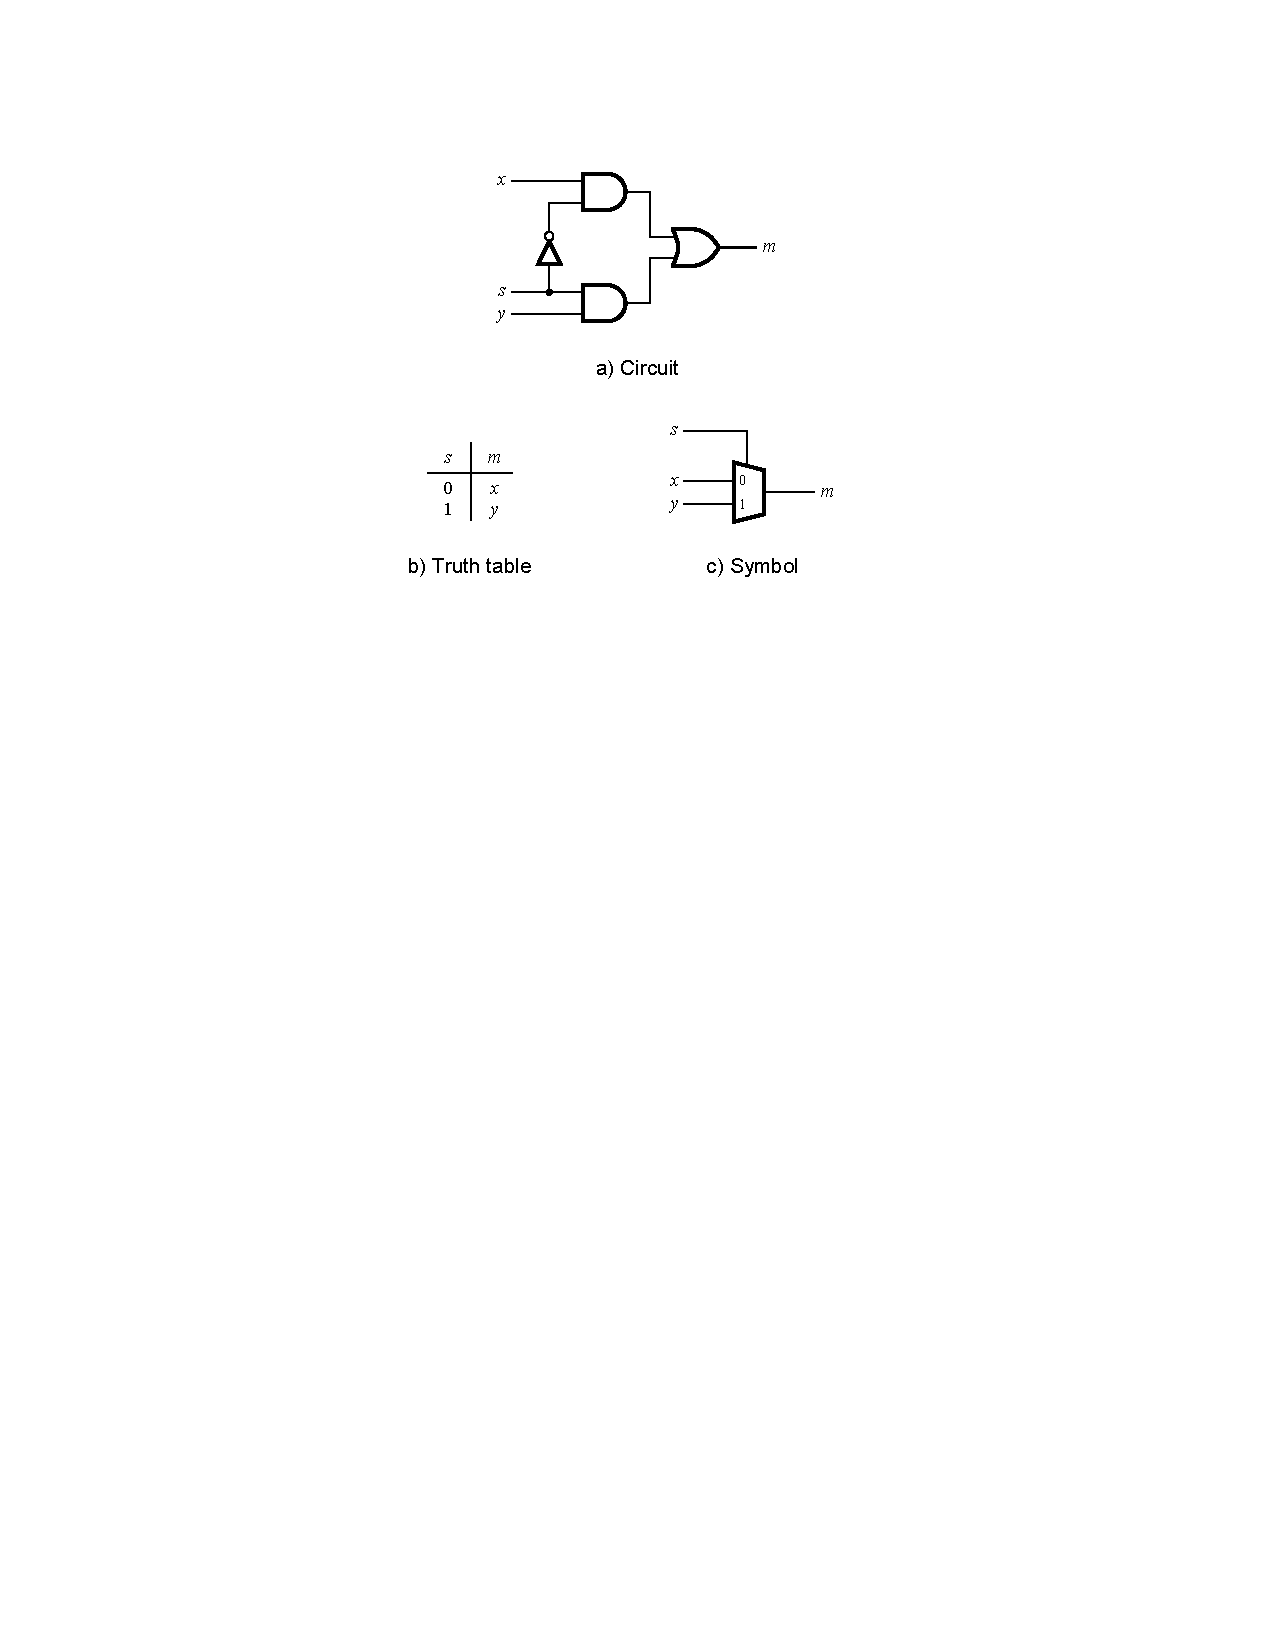
\includegraphics[scale=.8]{figures/figure2.pdf}
	\end{center}
	\caption{A 2-to-1 multiplexer.}
	\label{fig:2}
\end{figure}

The multiplexer can be described by the following Verilog statement:

\begin{center}
\begin{minipage}[t]{12.5 cm}
\begin{tabbing}
{\bf assign} m = ($\sim$s \& x) $\mid$ (s \& y);
\end{tabbing}
\end{minipage}
\end{center}

\newpage
You are to write a Verilog module that includes four
assignment statements like the one shown above to describe the circuit given 
in Figure~\ref{fig:3}$a$.
This circuit has two four-bit inputs, $X$ and $Y$, and produces the four-bit output
$M$. If $s=0$ then $M = X$, while if $s=1$ then $M=Y$. We refer to this circuit as a four-bit
wide 2-to-1 multiplexer. It has the circuit symbol shown in  Figure~\ref{fig:3}$b$, in which $X$,
$Y$, and $M$ are depicted as four-bit wires.

\begin{figure}[H]
	\begin{center}
		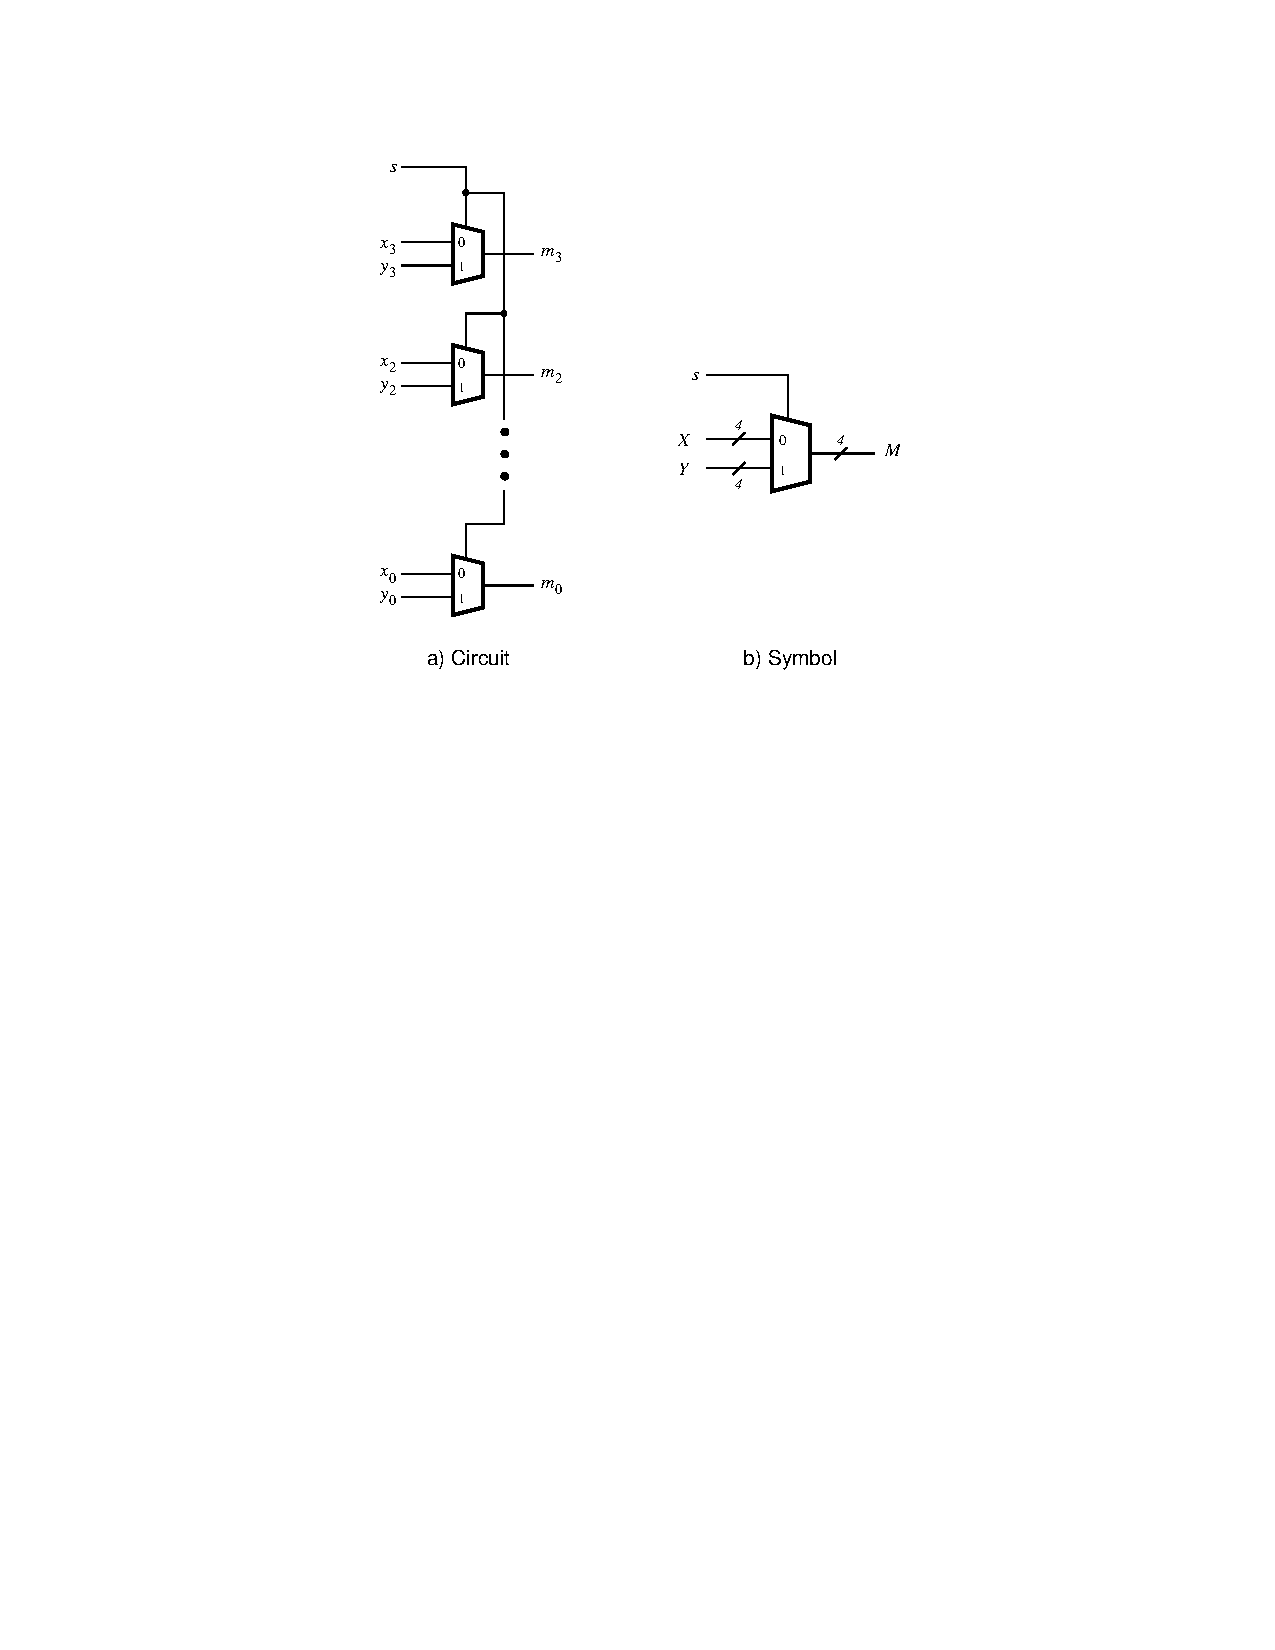
\includegraphics[scale=.8]{figures/figure3.pdf}
	\end{center}
\caption{A four-bit wide 2-to-1 multiplexer.}
\label{fig:3}
\end{figure}

Perform the steps listed below.
\begin{enumerate}
\item Create a new Quartus project for your circuit.
\item Include your Verilog file for the four-bit wide 2-to-1 multiplexer 
in your project. Use switch {\it SW}$_{9}$ as the $s$ input, switches
{\it SW}$_{3-0}$ as the $X$ input and 
{\it SW}$_{7-4}$ as the $Y$ input. Display the value of the input $s$ on {\it LEDR}$_9$,
connect the output $M$ to {\it LEDR}$_{3-0}$, and connect the unused LEDR lights to the constant value 0.
\item Include in your project the required pin assignments for your DE-series board. As discussed
in Part I, these assignments ensure that the ports of your Verilog code will use the pins 
on the FPGA chip that are connected to the {\it SW} switches and {\it LEDR} lights. 
\item Compile the project, generate a .qsf file in Quartus and upload it to the NO-IDE lab of LabsLand.
Test the functionality of the 
four-bit wide 2-to-1 multiplexer by toggling the switches and observing the LEDs.
\item For more info, if you have a FPGA chip, you can download the compiled circuit into the FPGA chip.
\end{enumerate}

\section*{Part III}
\addcontentsline{toc}{3}{Part III}
In Figure~\ref{fig:2} we showed a 2-to-1 multiplexer that selects between the 
two inputs {\it x} and {\it
y}. For this part consider a circuit in which the output {\it m} has to be selected from
four inputs $u$, $v$, $w$, and $x$. Part $a$ of  Figure~\ref{fig:4} shows how we can build the
required 4-to-1 multiplexer by using three 2-to-1 multiplexers. The circuit uses a 2-bit
select input $s_1 s_0$ and implements the truth table shown in Figure~\ref{fig:4}$b$. A circuit
symbol for this multiplexer is given in part $c$ of the figure. 

~\\
Recall from  Figure~\ref{fig:3} that a four-bit wide 2-to-1 multiplexer can be built 
by using four instances of a 2-to-1
multiplexer. Figure~\ref{fig:5} applies this concept to define a two-bit wide 4-to-1 
multiplexer. It contains two instances of the circuit in  Figure~\ref{fig:4}$a$.

\begin{figure}[H]
	\begin{center}
		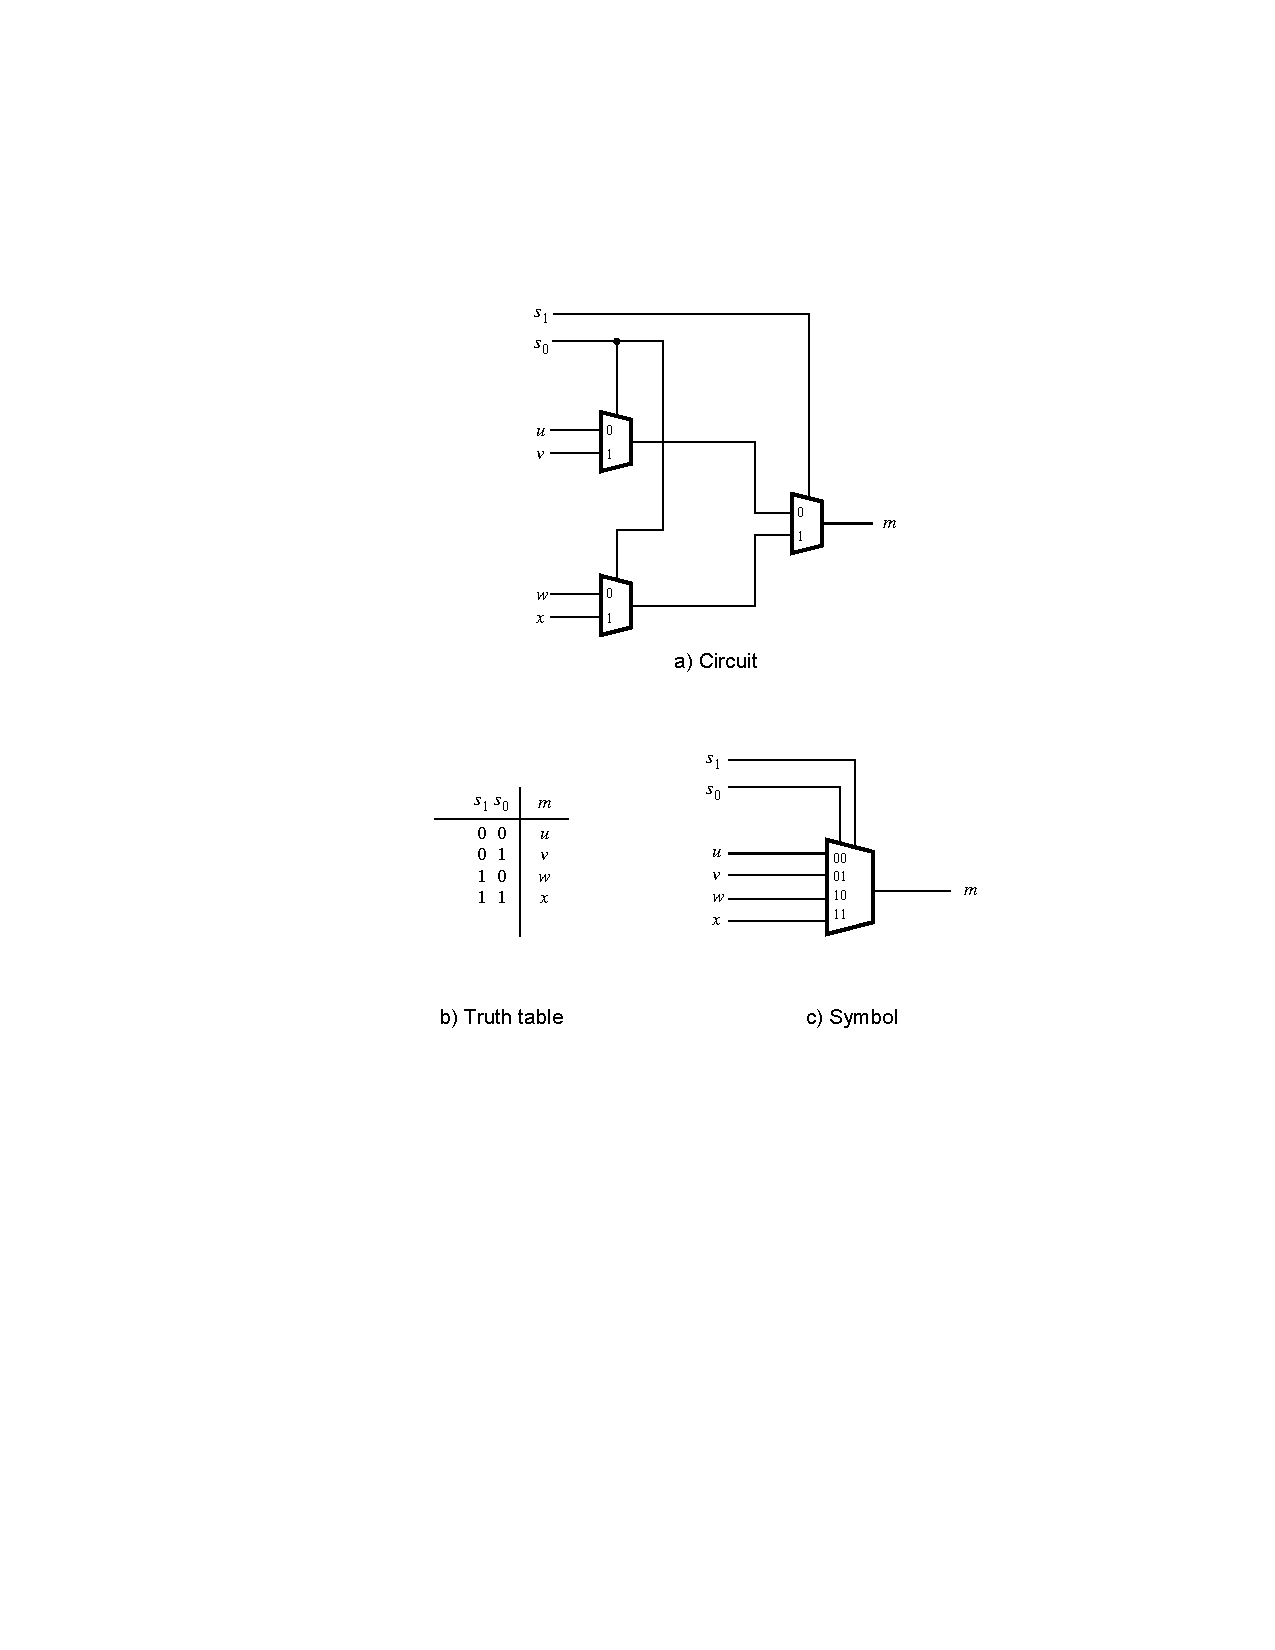
\includegraphics[scale=.8]{figures/figure4.pdf}
	\end{center}
\caption{A 4-to-1 multiplexer.}
\label{fig:4}
\end{figure}

\begin{figure}[H]
	\begin{center}
		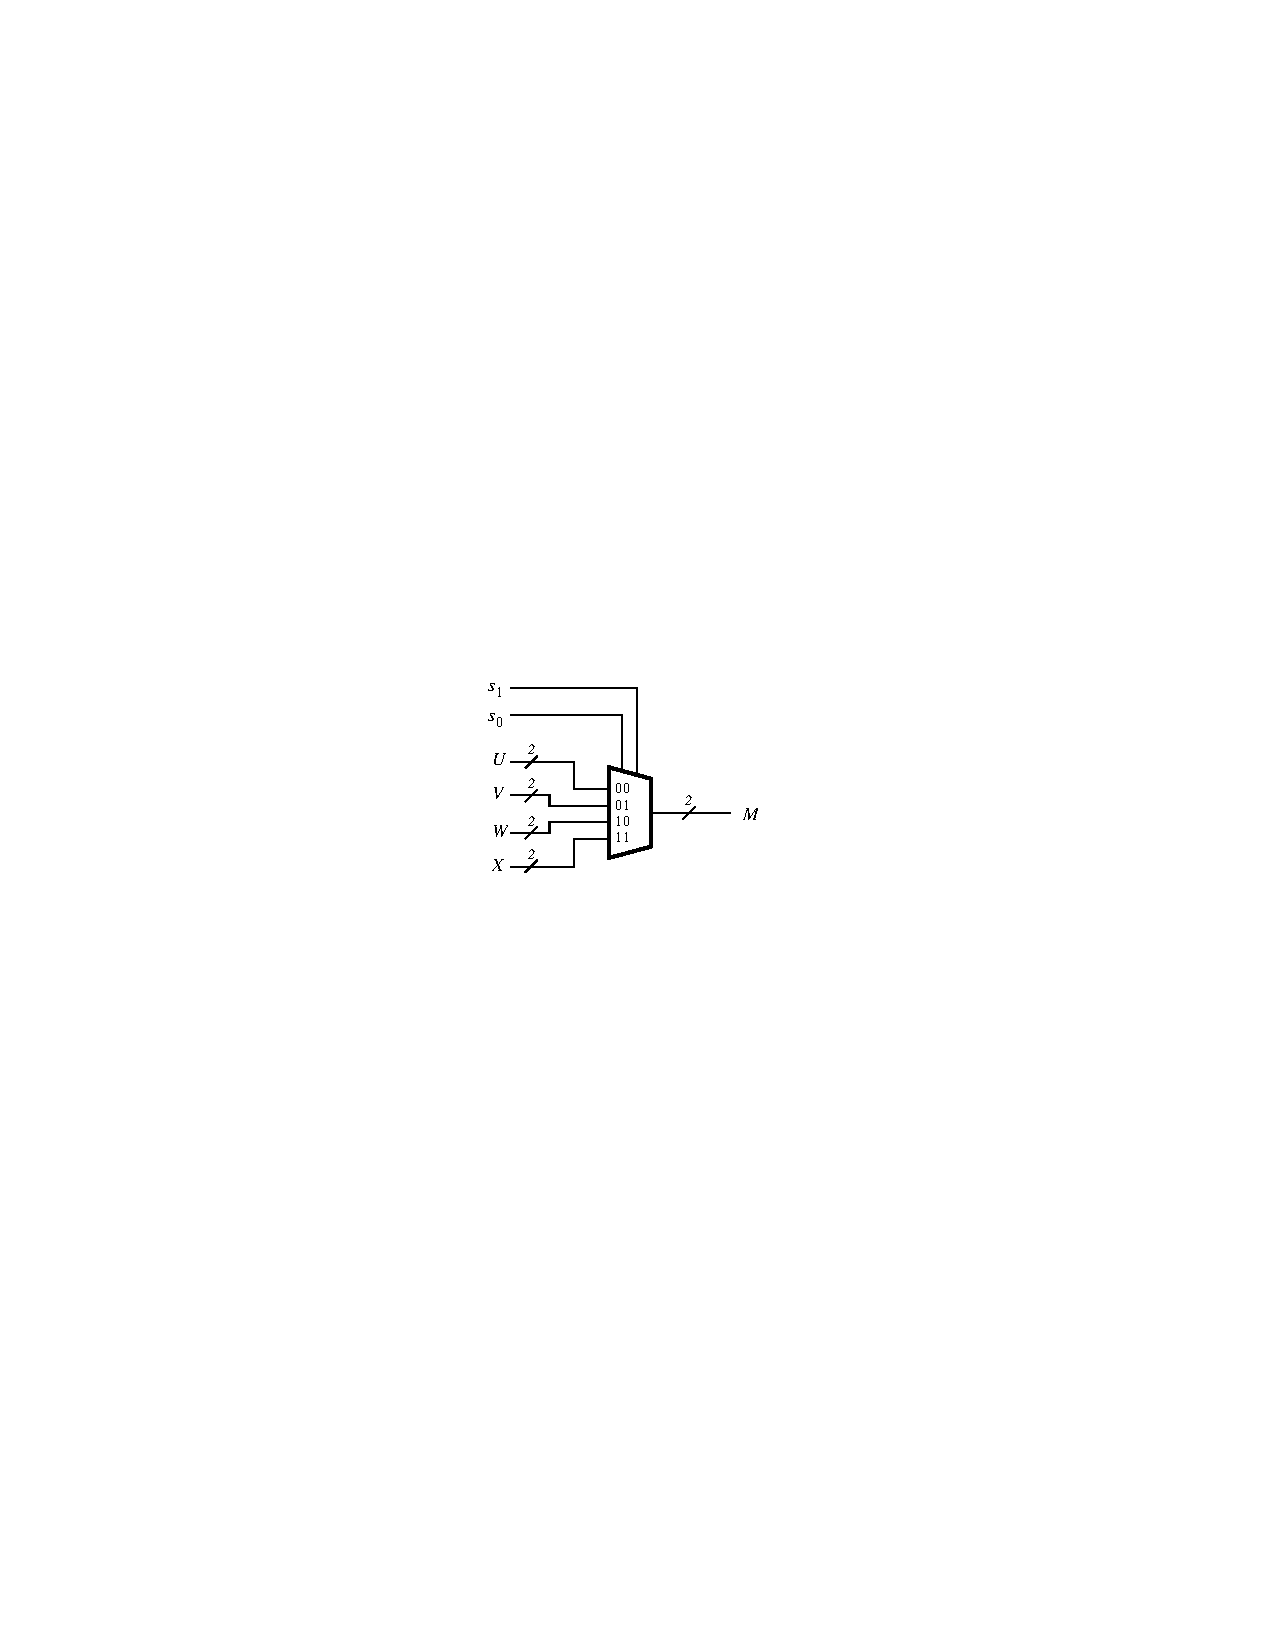
\includegraphics[]{figures/figure5.pdf}
	\end{center}
\caption{A two-bit wide 4-to-1 multiplexer.}
\label{fig:5}
\end{figure}

Perform the following steps to implement the two-bit wide 4-to-1 multiplexer.
\begin{enumerate}
\item Create a new Quartus project for your circuit.
\item Create a Verilog module for the two-bit wide 4-to-1 multiplexer. Connect its select
inputs to switches {\it SW}$_{9-8}$, and use switches SW$_{7-0}$ to
provide the four 2-bit inputs $U$ to $X$. Connect the 
output $M$ to the red lights {\it LEDR}$_{1-0}$.
\item Include in your project the required pin assignments for your DE-series board.
Compile the project.
\item Generate a .qsf file in Quartus and upload it to the NO-IDE lab of LabsLand. Test the functionality of the 
two-bit wide 4-to-1 multiplexer by toggling the switches and observing the LEDs. Ensure
that each of the inputs $U$ to $X$ can be properly selected as the output $M$.
\item For more info, if you have a FPGA chip, you can download the compiled circuit into the FPGA chip.
\end{enumerate}

\section*{Part IV}
\addcontentsline{toc}{4}{Part IV}
The objective of this part is to display a character on a 7-segment display.
The specific character displayed depends on a two-bit input.
Figure~\ref{fig:6} shows a {\it 7-segment decoder} module that has the two-bit input $c_1
c_0$. This decoder produces seven outputs that are used to display a character on a
7-segment display. Table~\ref{tab:codes} lists the characters that should be displayed for each
valuation of $c_1 c_0$ for your DE-series board. Note that in some cases the `blank' 
character is selected for code $11$.
~\\

The seven segments in the display are identified by the indices 0 to 6 shown in the
figure. Each segment is illuminated by driving it to the logic value 0. You are to write a
Verilog module that implements logic functions to activate
each of the seven segments.
Use only simple Verilog {\bf assign} statements in your code to specify each logic function using a
Boolean expression. 

\begin{figure}[H]
	\begin{center}
		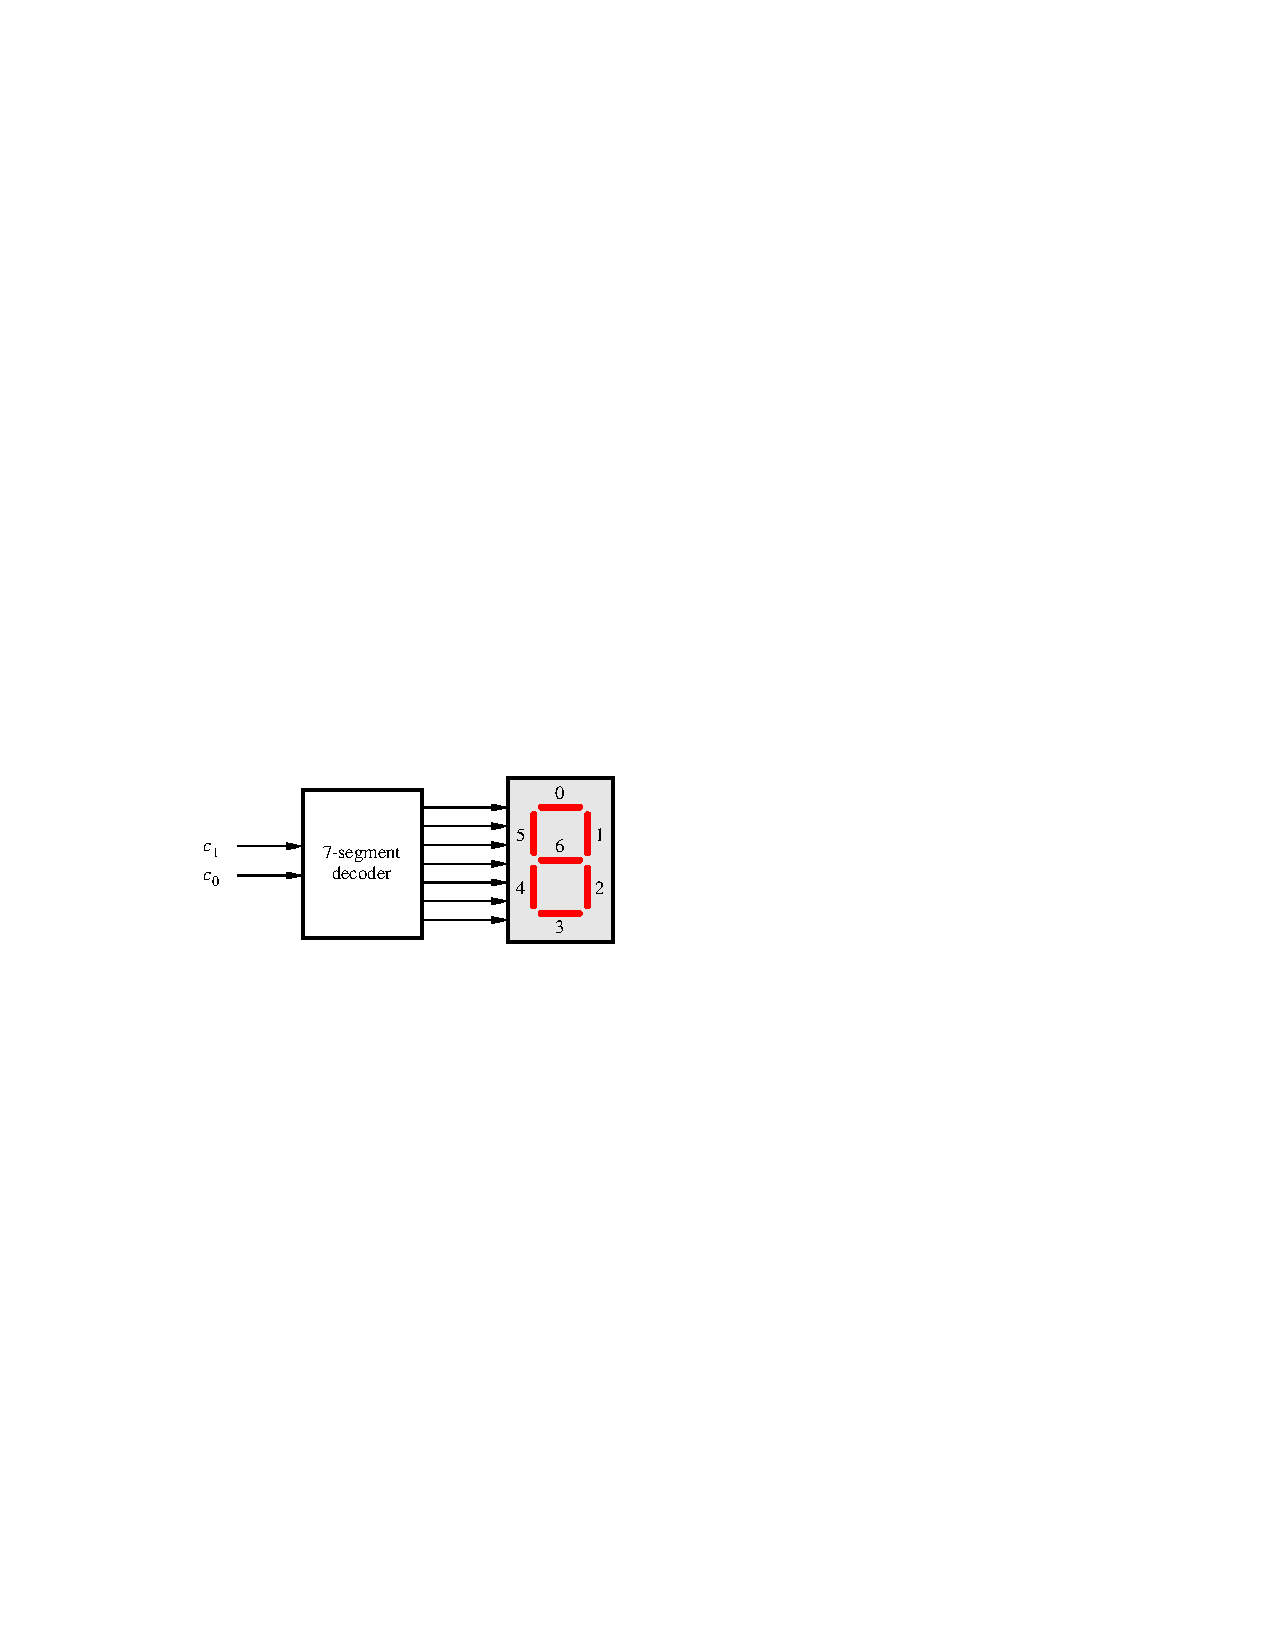
\includegraphics[]{figures/figure6.pdf}
	\end{center}
\caption{A 7-segment decoder.}
\label{fig:6}
\end{figure}

\begin{table}[H]
	\begin{center}
	\begin{tabular}{l | c | c | c | c}
	$c_1 c_0$ & DE10-Lite & DE0-CV & DE1-SoC & DE2-115 \\
	\hline
	{\rule[0mm]{0mm}{5mm}\hspace{0.75 mm} 00} & d & d & d & d \\
	\hspace{0.75 mm}
	01 & E & E & E & E \\
	\hspace{0.75 mm}
	10 & 1 & 0 & 1 & 2 \\
	\hspace{0.75 mm}
	11 & 0 & & & \\
	\end{tabular}
	\caption{Character codes for the DE-series boards.}
	\label{tab:codes}
	\end{center}
\end{table}

Perform the following steps:

\begin{enumerate}
\item Create a new Quartus project for your circuit.
\item Create a Verilog module for the 7-segment decoder. Connect the $c_1 c_0$ inputs
to switches {\it SW}$_{1-0}$, and connect the outputs of the decoder to the {\it HEX0} 
display on your DE-series board. The segments in this display are called 
{\it HEX0}$_0$, {\it HEX0}$_1$, $\ldots$, {\it HEX0}$_6$, corresponding to  Figure~\ref{fig:6}.
You should declare the 7-bit port 

\begin{center}
\begin{minipage}[t]{12.5 cm}
\begin{tabbing}
{\bf output} [0:6] HEX0;
\end{tabbing}
\end{minipage}
\end{center}

in your Verilog code so that the
names of these outputs match the corresponding names in your board's user manual and pin assignment file.
\item After making the required pin assignments, compile the project.
\item Generate a .qsf file in Quartus and upload it to the NO-IDE lab of LabsLand. Test the functionality of the 
circuit by toggling the {\it SW}$_{1-0}$ switches and observing the 7-segment display.
\item For more info, if you have a FPGA chip, you can download the compiled circuit into the FPGA chip.
\end{enumerate}

\newpage
\section*{Part V}
\addcontentsline{toc}{5}{Part V}
Consider the circuit shown in  Figure~\ref{fig:7}. It uses a two-bit wide 4-to-1 multiplexer to
enable the selection of four characters that are displayed on a 7-segment display. Using the
7-segment decoder from Part IV this circuit can display the characters d, E, 0, 1, 2, or `blank' 
depending on your DE-series board.
The character codes are set according to Table~\ref{tab:codes} by using the switches 
{\it SW}$_{7-0}$, and a specific character is selected for display by setting the
switches {\it SW}$_{9-8}$.
~\\

An outline of the Verilog code that represents this circuit is 
provided in  Figure~\ref{fig:8}. Note that we have
used the circuits from Parts III and IV as subcircuits in this code. You are to
extend the code in  Figure~\ref{fig:8} so that it uses four 7-segment displays rather 
than just one.  You will need to use four instances of each of the subcircuits. The
purpose of your circuit is to display any word on the four 7-segment displays that is 
composed of the characters in Table~\ref{tab:codes}, and be able to rotate this word in a 
circular fashion across the
displays when the switches {\it SW}$_{9-8}$ are toggled. As an example,
if the displayed word is dE10, then your circuit should produce the output patterns
illustrated in Table~\ref{tab:rotate}.

\begin{figure}[H]
	\begin{center}
		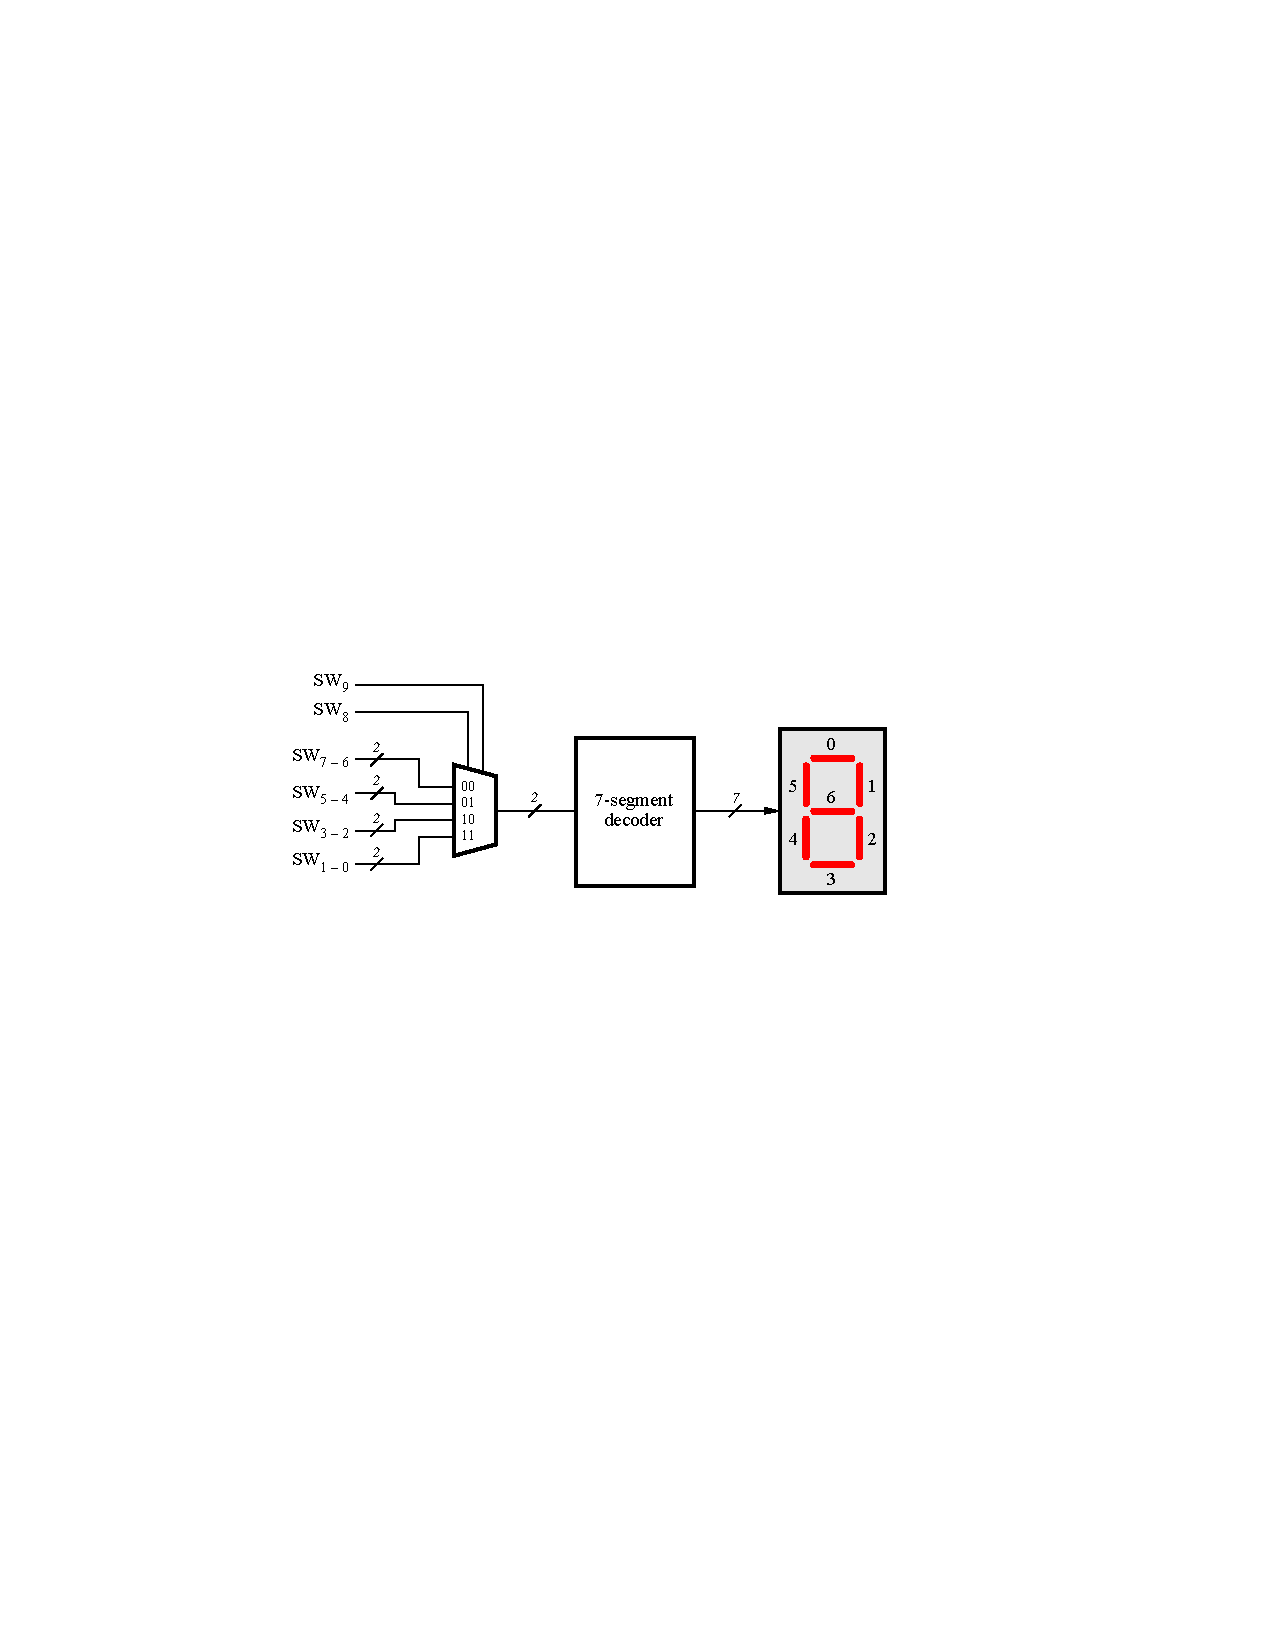
\includegraphics[]{figures/figure7.pdf}
	\end{center}
\caption{A circuit that can select and display one of four characters.}
\label{fig:7}
\end{figure}

\begin{figure}[ht]
\begin{center}
\begin{minipage}[t]{12.5 cm}
\begin{tabbing}
ZZ\={\bf output} [0:6] HEX3, HEX2, HEX1, HEX0;ZZ\=\kill
{\bf module} ~part5 (SW, LEDR, HEX0);\\
\>{\bf input} [9:0] SW;	\>// slide switches\\
\>{\bf output} [9:0] LEDR;	\>// red lights\\
\>{\bf output} [0:6] HEX0;	\>// 7-seg display\\
ZZ\=ZZ\=ZZ\=ZZ\=ZZ\=ZZ\=ZZ\=ZZ\=ZZ\=ZZ\=ZZ\kill
~\\
\>{\bf wire} [1:0] M0;\\
~\\
\>mux\_2bit\_4to1 U0 (SW[9:8], SW[7:6], SW[5:4], SW[3:2], SW[1:0], M0);\\
\>char\_7seg H0 (M0, HEX0);\\
\>$\ldots$\\
{\bf endmodule}\\
~\\
// implements a 2-bit wide 4-to-1 multiplexer\\
{\bf module} mux\_2bit\_3to1 (S, U, V, W, X, M);\\
\>{\bf input} [1:0] S, U, V, W, X;\\
\>{\bf output} [1:0] M;\\
\>$\ldots$ code not shown\\
~\\
{\bf endmodule}	\\
~\\
// implements a 7-segment decoder for d, E, 1 and 0\\
{\bf module} char\_7seg (C, Display);\\
\>{\bf input} [1:0] C;	\>\>\>\>\>\>\>\>// input code\\
\>{\bf output} [0:6] Display;	\>\>\>\>\>\>\>\>// output 7-seg code\\
\>$\ldots$ code not shown\\
~\\
{\bf endmodule}
\end{tabbing}
\end{minipage}
\end{center}
\caption{Verilog code for the circuit in  Figure~\ref{fig:7}.}.
\label{fig:8}
\end{figure}

\begin{table}[H]
\begin{minipage}[t]{12.5 cm}
\begin{center}
\begin{tabular}{c|cccc}
{\it SW}$_{9-8}$ & \multicolumn{4}{c}{Characters} \\
\hline
{\rule[0mm]{0mm}{5mm}00} & d & E & 1 & 0\\ 
01 & E & 1 & 0 & d\\
10 & 1 & 0 & d & E\\
11 & 0 & d & E & 1\\
\end{tabular}
\end{center}
\end{minipage}
\caption{Rotating the word dE10 on four displays.}
\label{tab:rotate}
\end{table}

Perform the following steps.
\begin{enumerate}
\item Create a new Quartus project for your circuit.
\item Include your Verilog module in the Quartus project. Connect the switches 
{\it SW}$_{9-8}$ to the select inputs of each of the four instances of the two-bit 
wide 4-to-1 multiplexers. Also connect {\it SW}$_{7-0}$ to each instance of the
multiplexers as required to produce the patterns of characters shown in Table~\ref{tab:codes}.
Connect the SW switches to the red lights LEDR, and connect the outputs of the four 
multiplexers to the 7-segment displays {\it HEX3}, {\it HEX2}, {\it HEX1}, and {\it HEX0}.
\item Include the required pin assignments for your DE-series board for all switches, LEDs, 
and 7-segment displays. Compile the project.
\item Generate a .qsf file in Quartus and upload it to the NO-IDE lab of LabsLand. Test the functionality of the 
circuit by setting the proper character codes on the switches SW$_{7-0}$ and then 
toggling {\it SW}$_{9-8}$ to observe the rotation of the characters.
\item For more info, if you have a FPGA chip, you can download the compiled circuit into the FPGA chip.
\end{enumerate}

\section*{Part VI}
\addcontentsline{toc}{6}{Part VI}
Extend your design from Part V so that is uses all 7-segment displays on your DE-series board.
Your circuit needs to display a three- or four-letter word, corresponding to Table 2,
using 'blank' characters for unused displays. Implement rotation of this word from right-to-left 
as indicated in Table~\ref{tab:rotate2} and Table~\ref{tab:rotate3}.
To do this, you will need to connect 6-to-1 multiplexers to each of six 7-segment display 
decoders for the DE10-Lite, DE0-CV and DE1-SoC. Note that for the DE10-Lite you will need
to use 3-bit codes for your characters, because five characters are needed when including
the 'blank' character (your 7-segment decoder will have to use 3-bit codes, and you will
need to use 3-bit wide 6-to-1 multiplexers).  For the DE2-115, you will need to connect 
8-to-1 multiplexers to each of the eight 7-segment display decoders. 
You will need to use three select lines for each of the multiplexers: connect the select lines 
to switches {\it SW}$_{9-7}$. In your Verilog code connect constants to the 6-to-1 (or
8-to-1) multiplexers that select each character, because there are not enough {\it SW} switches.

\begin{table}[h]
\begin{minipage}[t]{12.5 cm}
\begin{center}
\begin{tabular}{c|cccccc}
{\it SW}$_{9-7}$ & \multicolumn{6}{c}{Character pattern} \\
\hline
{\rule[0mm]{0mm}{5mm}000 } & & & d & E & 1 & 0 \\ 
001 & & d & E & 1 & 0 & \\
010 & d & E & 1 & 0 & & \\
011 & E & 1 & 0 & & & d\\
100 & 1 & 0 & & & d & E \\
101 & 0 & & & d  & E & 1 \\
\end{tabular}
\end{center}
\end{minipage}
\caption{Rotating the word dE10 on six displays.}
\label{tab:rotate2}
\end{table}

\clearpage

\begin{table}[ht]
\begin{minipage}[t]{12.5 cm}
\begin{center}
\begin{tabular}{c|cccccccc}
{\it SW}$_{9-7}$ & \multicolumn{6}{c}{Character pattern} \\
\hline
{\rule[0mm]{0mm}{5mm}000 } & & & & & & d & E & 2 \\ 
001 & & & & & d & E & 2 & \\
010 & & & & d & E & 2 & & \\
011 & & & d & E & 2 & & & \\
100 & & d & E & 2 & & & & \\
101 & d & E & 2 & & & & &  \\
110 & E & 2 & & & & & & d \\
111 & 2 & & & & & & d & E \\
\end{tabular}
\end{center}
\end{minipage}
\caption{Rotating the word dE2 on eight displays.}
\label{tab:rotate3}
\end{table}

Perform the following steps:
\begin{enumerate}
\item Create a new Quartus project for your circuit.
\item Include your Verilog module in the Quartus project. Connect the switches 
{\it SW}$_{9-7}$ to the select inputs of each instance of the 
multiplexers in your circuit. Connect constants in your Verilog code to the multiplexers 
as required to produce the patterns of characters shown in Table~\ref{tab:rotate2} or 
Table~\ref{tab:rotate3} depending on your DE-series board.
Connect the outputs of your multiplexers to the 7-segment displays {\it HEX5}, $\ldots$, 
{\it HEX0} of the DE10-Lite, DE0-CV and DE1-SoC or {\it HEX7}, $\ldots$, 
{\it HEX0} for the DE2-115.
\item Include the required pin assignments for your DE-series board for all switches, LEDs, 
and 7-segment displays. Compile the project.
\item Generate a .qsf file in Quartus and upload it to the NO-IDE lab of LabsLand. Test the functionality of the 
circuit by toggling {\it SW}$_{9-7}$ to observe the rotation of the characters.
\item For more info, if you have a FPGA chip, you can download the compiled circuit into the FPGA chip.
\end{enumerate}


%%%%%%%%%%%%%%%%%%%%%%%%%%%%%%%%%%%%%%%%
%%% FPGAcademy Copyright Information %%%
%%%%%%%%%%%%%%%%%%%%%%%%%%%%%%%%%%%%%%%%

%Always put the copyright on a new page (clear page), with some vertical space from top
\clearpage
\vspace{1in}

\noindent

Copyright {\copyright} FPGAcademy.org. All rights reserved. FPGAcademy and the 
FPGAcademy logo are trademarks of FPGAcademy.org.  This document is provided 
"as is", without warranty of any kind, express or implied, including but not 
limited to the warranties of merchantability, fitness for a particular purpose 
and noninfringement. In no event shall the authors or copyright holders be 
liable for any claim, damages or other liability, whether in an action of 
contract, tort or otherwise, arising from, out of or in connection with the 
document or the use or other dealings in the document.
~\\
~\\
**Other names and brands may be claimed as the property of others.


\end{document}
